\date{}
\title{}
\date{}
\usepackage[outputdir=latex.out]{minted}
\begin{document}
\begin{frame}
    \titlepage
\end{frame}


\makeatletter
\newenvironment<>{btHighlight}[1][]
{\begin{onlyenv}#2\begingroup\tikzset{bt@Highlight@par/.style={#1}}\begin{lrbox}{\@tempboxa}}
{\end{lrbox}\bt@HL@box[bt@Highlight@par]{\@tempboxa}\endgroup\end{onlyenv}}

\newcommand<>\btHL[1][]{%
  \only#2{\begin{btHighlight}[#1]\bgroup\aftergroup\bt@HL@endenv}%
}
\def\bt@HL@endenv{%
  \end{btHighlight}%   
  \egroup %
}
\tikzset{
    btHLbox/.style={
        fill=red!30,outer sep=0pt,inner xsep=1pt, inner ysep=0pt, rounded corners=3pt
    },
}
\newcommand{\bt@HL@box}[2][]{%
  \tikz[#1]{%
    \pgfpathrectangle{\pgfpoint{1pt}{0pt}}{\pgfpoint{\wd #2}{\ht #2}}%
    \pgfusepath{use as bounding box}%
    \node[text width={},draw=none,anchor=base west, btHLbox, minimum height=\ht\strutbox+1pt,#1]{\raisebox{1pt}{\strut}\strut\usebox{#2}};
  }%
}

\lst@CCPutMacro
    \lst@ProcessOther {"2A}{%
      \lst@ttfamily 
         {\raisebox{2pt}{*}}% used with ttfamily
         {\raisebox{2pt}{*}}}% used with other fonts
    \@empty\z@\@empty

\lstdefinelanguage
   [x8664gas]{Assembler}     % add a "x64" dialect of Assembler
   [x86masm]{Assembler} % based on the "x86masm" dialect
   % with these extra keywords:
   {morekeywords={CDQE,CQO,CMPSQ,CMPXCHG16B,JRCXZ,LODSQ,MOVSXD,%
                  POPFQ,PUSHFQ,SCASQ,STOSQ,IRETQ,RDTSCP,SWAPGS,.TEXT,.STRING,.ASCIZ,%
                  BEQ,LW,SW,LB,SB,ADDIU,J,BEQZ,BNEZ,BNE,%
                  MOVUPD,MULPD,MOVSD,MULSD,%
                  SHLADD,MOV,CMP.LT,TBIT.NZ,BR.RET.SPTK.MANY,%
                  ADDQ,POPQ,PUSHQ,RRMOVQ,MRMOVQ,RMMOVQ,IRMOVQ,%
                  <-,LL,SC,ADDI,ADDL,VMOVDQA,ADDQ,CMPL,JB,JBE,MOVL,CLTQ,%
                  MOVW,PUSHW,MOV,ADD,SUB,INT,PUSH,MOV,ADD,REP,MOVSB,%
                  TESTQ,CMPQ,MOVL,MOVQ,ADDQ,JMPQ,XORQ,%
                  LEAQ,LEAL,LEA,RETQ,RET,POPL,POPW,PUSHL,PUSHW,%
                  LEAW,%
                  SUBQ,SYSCALL,.ASCII,CALLQ,MOVSLQ,JMP,ANDQ,SHRQ,MOVB,INCQ,TESTL,XORL,%
                  SHRL,LEAL,SARL,SUBL,IMULL,IMULQ,MOVDQU,PADDD,XORL,%
                  MOVZBL,MOVZB,SHRB,SRAL,SHRL,ANDL,%
                  CMOVNS,SRAL,SRAQ,MOVZBW,MOVZBQ,%
                  PADDW,PADDQ,MODUPS,MOVAPD,%
                  MOVL,RET,.GLOBL,%
		  PAUSE,LFENCE,JMP,%
                  },
    deletekeywords={eax,ebx,sp,si,cx,di,ds,cs,es,fs,dx,ax,bx,al,esi,ebp,ecx,rip,eip,edx,edi,rdi,esp},
    deletekeywords=[2]{size},
    alsoletter={\%},
    alsoother={()},
    emphstyle={\color{violet!50!black}},
    emph={\%rax,\%rbx,\%rcx,\%rdx,\%r8,\%r9,\%r10,\%r11,\%r12,\%r13,\%r14,\%r15,\%eax,\%ebx,\%sp,\%si,\%cx,\%di,\%ds,\%cs,\%es,\%fs,\%dx,\%ax,\%bx,\%al,\%esi,\%ebp,\%ecx,\%rip,\%eip,\%edx,\%edi,\%rdi,\%esp,\%rsp},
    %moreemph={eax,ebx,sp,si,cx,di,ds,cs,es,fs,dx,ax,bx,al,esi,ebp,ecx,rip,eip,edx,edi,rdi,esp},
    morecomment=[l]{\#},
    morecomment=[l]{\/\/},
    morecomment=[s]{/*}{*/},
    sensitive=false,
    keepspaces=true} % et

\lstalias[]{myasm}[x8664gas]{Assembler}

\lstdefinelanguage{JavaScript}{
  keywords={typeof, new, true, false, catch, function, return, null, catch, switch, var, if, in, while, do, else, case, break},
  ndkeywords={class, export, boolean, throw, implements, import, this},
  sensitive=false,
  comment=[l]{//},
  morecomment=[s]{/*}{*/},
  morestring=[b]',
  morestring=[b]"
}

\newcommand{\keywordstyle}{\sourcecodeprolight\bfseries\color{blue!30!black}}
\newcommand{\stringstyle}{\color{blue!20!black}\ttfamily}

\lstset{
    language=C,
    basicstyle=\sourcecodepro\EmptyMapping,
    escapechar=`,
    keywordstyle=\keywordstyle\EmptyMapping,
    identifierstyle=\sourcecodepro\EmptyMapping,
    numberstyle=\small\color{black!70},
    commentstyle=\color{red!60!black}\ttfamily\itshape,
    stringstyle=\color{blue!20!black}\ttfamily,
    ndkeywordstyle=\bfseries\color{blue!30!black},
    upquote=true,
}



\lstdefinestyle{medium}{
    basicstyle=\sourcecodepro\EmptyMapping\fontsize{12}{13}\selectfont,
    keywordstyle=\sourcecodepro\EmptyMapping\fontsize{12}{13}\selectfont\keywordstyle,
}

\lstdefinestyle{small}{
    basicstyle=\sourcecodepro\EmptyMapping\small,
    keywordstyle=\sourcecodepro\EmptyMapping\small\keywordstyle,
}

\lstdefinestyle{smaller}{
    basicstyle=\sourcecodepro\EmptyMapping\fontsize{11}{12}\selectfont,
    keywordstyle=\sourcecodepro\EmptyMapping\fontsize{11}{12}\selectfont\keywordstyle,
}

\lstdefinestyle{size105}{
    basicstyle=\sourcecodepro\EmptyMapping\fontsize{10.5}{11.5}\selectfont,
    keywordstyle=\sourcecodepro\EmptyMapping\fontsize{10.5}{11.5}\selectfont\keywordstyle,
}

\lstdefinestyle{size10}{
    basicstyle=\sourcecodepro\EmptyMapping\fontsize{10}{11}\selectfont,
    keywordstyle=\sourcecodepro\EmptyMapping\fontsize{10}{11}\selectfont\keywordstyle,
}

\lstdefinestyle{size9}{
    basicstyle=\sourcecodepro\EmptyMapping\fontsize{9}{10}\selectfont,
    keywordstyle=\sourcecodepro\EmptyMapping\fontsize{9}{10}\selectfont\keywordstyle,
}
\lstdefinestyle{size8}{
    basicstyle=\sourcecodepro\EmptyMapping\fontsize{8}{9}\selectfont,
    keywordstyle=\sourcecodepro\EmptyMapping\fontsize{8}{9}\selectfont\keywordstyle,
}



\lstdefinestyle{script}{
    basicstyle=\sourcecodepro\EmptyMapping\scriptsize,
    keywordstyle=\sourcecodepro\EmptyMapping\scriptsize\bfseries,
}




\begin{frame}{last time}
    \begin{itemize}
    \item `fat pointer'-based bounds-checking
        \begin{itemize}
        \item have pointers include bounds of object/array
        \item can check on \textit{pointer dereference}
        \end{itemize}
    \item unfortunate C programming practices that break fat pointers
        \begin{itemize}
        \item converting pointers to ints and back
        \item converting pointer to Inner struct to Outer struct
        \end{itemize}
    \item baggy bounds check
        \begin{itemize}
        \item store bounds in lookup table
        \item check \textit{pointer arithmetic}
        \item (can't allow out-of-bounds pointer --- lost bounds information)
        \item make things multiple of power of two to speed up checks
        \item (at cost of a bunch of extra space)
        \end{itemize}
    \end{itemize}
\end{frame}

\begin{frame}{on SANDBOX (1)}
    \begin{itemize}
    \item will set filter \textit{after} worker program starts
        \begin{itemize}
        \item don't need to allow system calls needed for program startup only
        \end{itemize}
    \item okay for your program to abort on invalid operation
    \vspace{.5cm}
    \item IPC library aborts on communication problem
        \begin{itemize}
        \item choice I made because I thought people wouldn't check return values
        \end{itemize}
    \end{itemize}
\end{frame}


\begin{frame}{on SANDBOX (2)}
    \begin{itemize}
    \item on strace
        \begin{itemize}
        \item I think it's easiest to use strace on original program or test program that just calls dadasubst (since less going on)
        \item if using -f: lines prefixed with process IDs
        \item could figure out which PID is which by, e.g., outputting something and looking for it
        \item probably strace will show something when filter gets tripped
        \end{itemize}
    \end{itemize}
\end{frame}

\begin{frame}{on SANDBOX (3)}
    \begin{itemize}
    \item linking libseccomp -- \texttt{-lseccomp} when making executable
    \end{itemize}
\end{frame}

\begin{frame}{on CHALLENGE (1)}
    \begin{itemize}
    \item complete any 5 of 7 challenges
    \item your goal: create attackX.py (or .c or etc.), so that
        \begin{itemize}
        \item \texttt{python attackX.py exploit.dat}
        \item (get new copy of challengeX.exe)
        \item \texttt{setarch -RL env - ./challengeX.exe <exploit.dat}
        \end{itemize}
    \item terminates normally and produces output saying you passed the challenge
        \begin{itemize}
        \item (more details in the assignment writeup)
        \end{itemize}
    \end{itemize}
\end{frame}

\begin{frame}{on CHALLENGE (2)}
    \begin{itemize}
    \item can complete any 5 of 7 for full credit
        \begin{itemize}
        \item 20\% credit for each completed, no extra credit
        \item (any partial credit will be based on best 5 submitted)
        \end{itemize}
    \item will have challenges numbered in my rough guess about difficulty
        \begin{itemize}
        \item my guess may be wrong
        \item my guess may assume you make good (educated) guess about what strategy to use
        \end{itemize}
    \item will supply example solutions to prior attack-like assignments
    \item some challenges will come with source code/README
    \end{itemize}
\end{frame}

\begin{frame}{schedule note}
    \begin{itemize}
    \item haven't been keeping schedule page up-to-date, sorry!
    \item should be better now
    \end{itemize}
\end{frame}

\begin{frame}{future classes plan}
    \begin{itemize}
    \item bounds-checking (today?)
        \begin{itemize}
        \item AddressSanitizer, valgrind memchcek
        \end{itemize}
    \item control-flow integrity (CFI)
        \begin{itemize}
        \item check that calls/return go to `valid' locations
        \item what ENDBR64 is about
        \end{itemize}
    \item if time --- cross-site scripting (XSS) mitigations and same-origin policy (SOP)
        \begin{itemize}
        \item Content-Security-Policy
        \item cookie flags (secure; HTTPOnly; \ldots)
        \item restrictions on requests between webpages (
        \end{itemize}
    \item Q: should I cut down/move CFI stuff and prioritize XSS/SOP?
    \end{itemize}
\end{frame}

\section{baggy bounds con't}
\subsection{checks using table}
\usetikzlibrary{calc}
\begin{frame}{baggy bounds check: added code}
    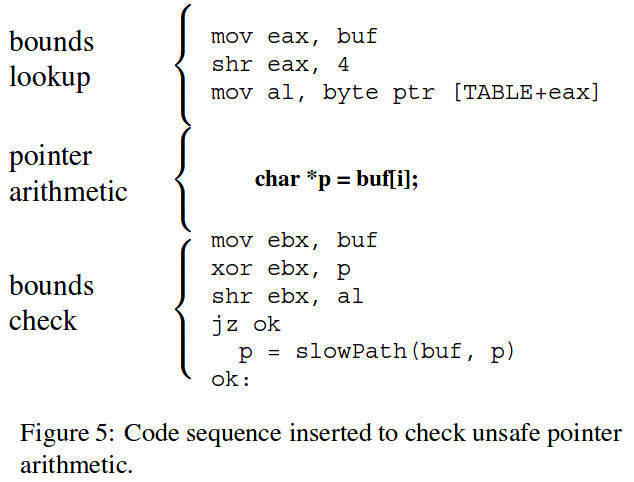
\includegraphics[width=0.6\textwidth]{../bounds/bb-bounds-check}
\end{frame}

\begin{frame}[fragile,label=addedCode]{baggy bounds check: added code}
    \lstset{language=myasm,style=small}
    \begin{lstlisting}
/* bounds lookup */
    mov buf, %rax
    shr %rax, 4
    mov LOOKUP_TABLE(%rax), %al
/* array element address computation */
    ...    // `\textbf{\textit{char * p = buf[i];}}`
/* bound check */
    mov buf, %rbx
    xor p, %rbx
    shr %al, %rbx
    jz  ok
    ...    // handle possible violation
ok:
\end{lstlisting}

    \imagecredit{adapted from paper figure}
\end{frame}

\begin{frame}{avoiding checks}
    \begin{itemize}
        \item code not added if not array/pointer accesses to object
        \item code not added when pointer accesses ``obviously'' safe
            \begin{itemize}
            \item author's implementation: only checked within function
            \end{itemize}
    \end{itemize}
\end{frame}



\subsection{exercise: overhead estimating?}
\begin{frame}<1>[fragile,label=bbOverheadExer1]{exercise: overhead of baggy bounds (1)}
\begin{itemize}
\item suppose program allocates:
    \begin{itemize}
    \item 1000 100 byte objects
    \item 1 10000 byte object
    \end{itemize}
\item using baggy bounds, estimate:
    \begin{itemize}
    \item space required for padding
        \begin{itemize}
        \item<2-> $(128-100)\cdot 1000 + (16384 - 10000)) = 34384$
        \end{itemize}
    \item space required for table
        \begin{itemize}
        \item<2-> $(128\cdot 1000 + 16384) \div 16 = 9024$
        \end{itemize}
    \end{itemize}
\end{itemize}
\end{frame}

\iftoggle{heldback}{}{\againframe<2>{bbOverheadExer1}}

\begin{frame}[fragile,label=bbOverheadExer2]{exercise: overhead of baggy bounds (2)}
\begin{lstlisting}[language=C,style=smaller]
char *strcat(char *d, char *s) {
    int i;
    for (i = 0; s[i] != '\0'; i += 1) {
        d[i] = s[i]; 
    }
    d[i] = '\0';
    return d;
}
\end{lstlisting}
\begin{itemize}
\item estimate:
\begin{itemize}
\item number of bounds checks needed
\item very rough number of instructions run w/o bounds check
\end{itemize}
\item thought question: \\
with bounds checking, what's fastest possible code?
\end{itemize}
\end{frame}


\subsection{alternative: pointer tagging}

\begin{frame}{alternate approach: pointer tagging}
    \begin{itemize}
        \item some bits of \myemph{address} are size 
        \begin{itemize}
        \item replaces table entry/lookup
        \end{itemize}
    \item change code to allocate objects this way
    \item works well on 64-bit --- plenty of addresses to use
    \end{itemize}
    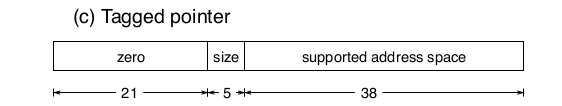
\includegraphics[width=0.8\textwidth]{../bounds/baggy-bounds-tagging}
\end{frame}



\subsection{performance?}

\begin{frame}{baggy bounds performance}
    \begin{itemize}
        \item table: 4--72\% time overhead (depends on benchmark suite)
        \item table: 11--21\% space overhead (depends on benchmark suite)
        \item tagged pointers: slightly better on average
    \end{itemize}
\end{frame}

\begin{frame}{baggy bounds performance}
    \begin{center}
    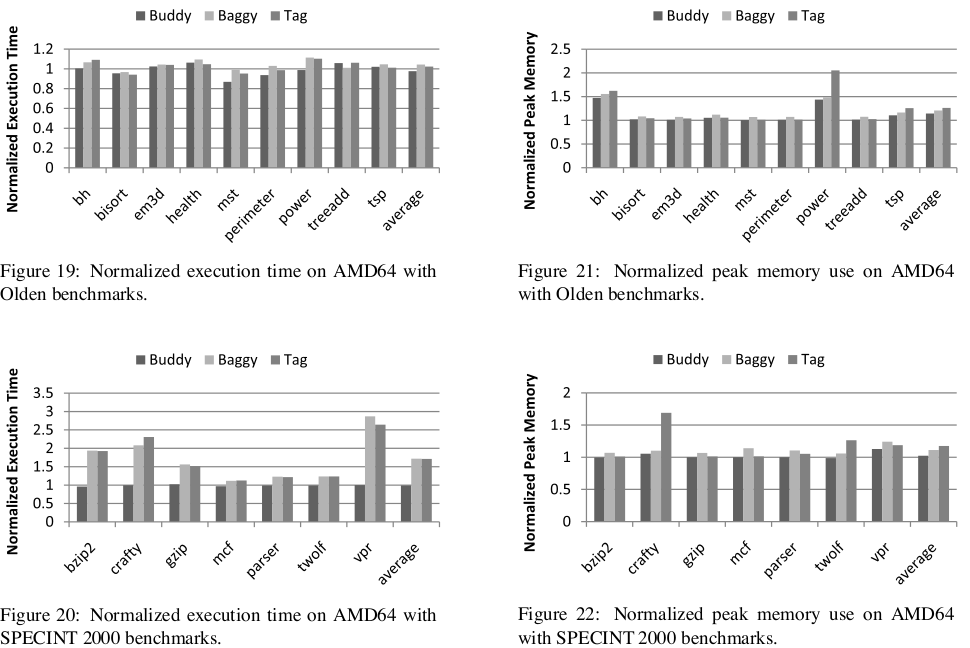
\includegraphics[height=0.8\textheight]{../bounds/baggy-bounds-perf}
    \end{center}
\end{frame}



\subsection{problem: pointers within objects}
% FIXME
\begin{frame}[fragile,label=withinObj]{problem: within object}
\begin{lstlisting}
struct foo {
    char buffer[1024];
    int *pointer;
};
struct foo array_of_foos[1024];
...
char *p = &array_of_foos[4].buffer[4]
\end{lstlisting}
\begin{itemize}
\item exercise: what are the bounds for p?
\end{itemize}
\end{frame}


\subsection{corner cases}

\begin{frame}[fragile,label=unfortunateCProgF2C]{unfortunate things C programmers do (4)}
in code generated by f2c (Fortran to C translator) \\
{\scriptsize (cleaned up slightly)}
\begin{lstlisting}[language=C,style=small]
float sum(int size, float *arr) {
    arr = arr - 1; /* <-- deliberately out-of-bounds pointer */
    float result = 0.f;
    for (i = 1; i <= size; ++i) {
        result += arr[i]
    }
    return result;
}
\end{lstlisting}
\end{frame}



\section{AddressSanitizer}

\begin{frame}{AddressSanitizer}
    \begin{itemize}
    \item like baggy bounds:
        \begin{itemize}
        \item big lookup table
        \item lookup table set by memory allocations
        \item compiler modification: change stack allocations
        \end{itemize}
    \item unlike baggy bounds:
        \begin{itemize}
        \item check reads/writes (instead of pointer computations)
        \item only detect errors that read/write \myemph{between objects}
        \item object sizes not padded to power of two
        \item table has info for every single byte (more precise)
        \end{itemize}
    \end{itemize}
\end{frame}




\subsection{ASan's added check}

\begin{frame}[fragile,label=asanVBounds]{adding bounds-checking example}
\lstset{
    language=C++,
    style=small,
    moredelim={**[is][\btHL<2>]{~2~}{~end~}},
}
\begin{lstlisting}
void vulnerable(long value, int offset) {
    long array[10] = {1,2,3,4,5,6,7,8,9,10};
    // generated code: (added by AddressSanitizer)
    ~2~if (!lookup_table[&array[offset]] == VALID) FAIL();~end~
    array[offset] = value;
    do_something_with(array);
}
\end{lstlisting}
    \begin{itemize}
        \item AddressSanitizer: crashes only if \lstinline|array[offset]| isn't part of any object
            \begin{itemize}
            \item but no extra space --- single-byte precision
            \end{itemize}
    \end{itemize}
\end{frame}



\subsection{stack layout}
\usetikzlibrary{arrows.meta,matrix,patterns}
\tikzset{
    stackBox/.style={very thick},
    allocBox/.style={dashed,very thick,fill=blue!20},
    onStack/.style={thick},
    frameOne/.style={fill=blue!15},
    frameTwo/.style={fill=red!15},
    markLine/.style={blue!50!black},
    markLineB/.style={red!90!black},
    hiLine/.style={red!90!black},
}
\begin{frame}[fragile,label=asanStackLayout]{AddressSanitizer stack layout}
    \begin{tikzpicture}
        \begin{scope}[x=1.7cm]
    \draw[stackBox] (0, 0) rectangle (5, -6);
            \draw[onStack] (0, 0) rectangle (5, -.5)
        node[midway] (arrayLoc) { return address (for \texttt{vulernable()}) };
    \begin{visibleenv}<2>
        \node[anchor=west] at (5.25, -.25) { $\approx$ \tt array[0x13]};
        \node[anchor=west] at (5.25, -3.75) { $\approx$ \tt array[0xa]};
    \end{visibleenv}
    \draw[onStack] (0, -.5) rectangle (5, -1)
        node[midway] { saved \tt\%rbp };
    \draw[onStack] (0, -1) rectangle (5, -1.5)
        node[midway] { saved \tt\%r13 };
    \draw[onStack] (0, -1.5) rectangle (5, -2)
        node[midway] { saved \tt\%r12 };
    \draw[onStack] (0, -2) rectangle (5, -2.5)
        node[midway] { saved \tt\%rbx };
    \draw[onStack,pattern=north west lines,pattern color=red] (0, -2.5) rectangle (5, -4)
        node[midway,fill=white] { ``red zone'' };
    \draw[onStack] (0, -4) rectangle (5, -6)
        node[midway,fill=white] { \tt array };
            \draw[onStack,dashed] (0, -4) rectangle (5, -4.5) node[midway] {\tt array[9]};
            \begin{visibleenv}<3>
            \matrix[tight matrix,
                nodes={text width=3cm,font=\small\tt},anchor=north west,label={north:lookup table}] (tbl) at (6, -2) {
                valid \\ valid  \\ valid \\ valid \\ valid \\ invalid \\ invalid \\
                invalid \\ invalid \\ valid \\ valid \\ \ldots \\
            };
                \draw[thick,-Latex] (5, -.25) -- (tbl-1-1.west);
                \draw[thick,-Latex] (5, -.75) -- (tbl-2-1.west);
            \end{visibleenv}
    \draw[thick,-Latex] (5.15, -6) --++ (0, 2);
        \end{scope}
    \end{tikzpicture}
\end{frame}





\section{AddressSanitizer}

\begin{frame}{AddressSanitizer}
    \begin{itemize}
    \item like baggy bounds:
        \begin{itemize}
        \item big lookup table
        \item lookup table set by memory allocations
        \item compiler modification: change stack allocations
        \end{itemize}
    \item unlike baggy bounds:
        \begin{itemize}
        \item check reads/writes (instead of pointer computations)
        \item only detect errors that read/write \myemph{between objects}
        \item object sizes not padded to power of two
        \item table has info for every single byte (more precise)
        \end{itemize}
    \end{itemize}
\end{frame}




\subsection{ASan's added check}

\begin{frame}[fragile,label=asanVBounds]{adding bounds-checking example}
\lstset{
    language=C++,
    style=small,
    moredelim={**[is][\btHL<2>]{~2~}{~end~}},
}
\begin{lstlisting}
void vulnerable(long value, int offset) {
    long array[10] = {1,2,3,4,5,6,7,8,9,10};
    // generated code: (added by AddressSanitizer)
    ~2~if (!lookup_table[&array[offset]] == VALID) FAIL();~end~
    array[offset] = value;
    do_something_with(array);
}
\end{lstlisting}
    \begin{itemize}
        \item AddressSanitizer: crashes only if \lstinline|array[offset]| isn't part of any object
            \begin{itemize}
            \item but no extra space --- single-byte precision
            \end{itemize}
    \end{itemize}
\end{frame}



\subsection{stack layout}
\usetikzlibrary{arrows.meta,matrix,patterns}
\tikzset{
    stackBox/.style={very thick},
    allocBox/.style={dashed,very thick,fill=blue!20},
    onStack/.style={thick},
    frameOne/.style={fill=blue!15},
    frameTwo/.style={fill=red!15},
    markLine/.style={blue!50!black},
    markLineB/.style={red!90!black},
    hiLine/.style={red!90!black},
}
\begin{frame}[fragile,label=asanStackLayout]{AddressSanitizer stack layout}
    \begin{tikzpicture}
        \begin{scope}[x=1.7cm]
    \draw[stackBox] (0, 0) rectangle (5, -6);
            \draw[onStack] (0, 0) rectangle (5, -.5)
        node[midway] (arrayLoc) { return address (for \texttt{vulernable()}) };
    \begin{visibleenv}<2>
        \node[anchor=west] at (5.25, -.25) { $\approx$ \tt array[0x13]};
        \node[anchor=west] at (5.25, -3.75) { $\approx$ \tt array[0xa]};
    \end{visibleenv}
    \draw[onStack] (0, -.5) rectangle (5, -1)
        node[midway] { saved \tt\%rbp };
    \draw[onStack] (0, -1) rectangle (5, -1.5)
        node[midway] { saved \tt\%r13 };
    \draw[onStack] (0, -1.5) rectangle (5, -2)
        node[midway] { saved \tt\%r12 };
    \draw[onStack] (0, -2) rectangle (5, -2.5)
        node[midway] { saved \tt\%rbx };
    \draw[onStack,pattern=north west lines,pattern color=red] (0, -2.5) rectangle (5, -4)
        node[midway,fill=white] { ``red zone'' };
    \draw[onStack] (0, -4) rectangle (5, -6)
        node[midway,fill=white] { \tt array };
            \draw[onStack,dashed] (0, -4) rectangle (5, -4.5) node[midway] {\tt array[9]};
            \begin{visibleenv}<3>
            \matrix[tight matrix,
                nodes={text width=3cm,font=\small\tt},anchor=north west,label={north:lookup table}] (tbl) at (6, -2) {
                valid \\ valid  \\ valid \\ valid \\ valid \\ invalid \\ invalid \\
                invalid \\ invalid \\ valid \\ valid \\ \ldots \\
            };
                \draw[thick,-Latex] (5, -.25) -- (tbl-1-1.west);
                \draw[thick,-Latex] (5, -.75) -- (tbl-2-1.west);
            \end{visibleenv}
    \draw[thick,-Latex] (5.15, -6) --++ (0, 2);
        \end{scope}
    \end{tikzpicture}
\end{frame}



\subsection{can't change object layout?}
\usetikzlibrary{arrows.meta,patterns,shapes.misc}
\tikzset{
    stackBox/.style={very thick},
    allocBox/.style={dashed,very thick,fill=blue!20},
    on stack/.style={thick},
    frameOne/.style={fill=blue!15},
    frameTwo/.style={fill=red!15},
    markLine/.style={blue!50!black},
    markLineB/.style={red!90!black},
    hiLine/.style={red!90!black},
}

\begin{frame}[fragile,label=changeObjLayout]{changing object layout?}
\begin{lstlisting}
struct string_list {
    char data[100];
    struct string_list *prev;
    struct string_list *next;
};
\end{lstlisting}
\begin{tikzpicture}[overlay,remember picture]
\node[anchor=south] at (2.5, 0) {actual layout};
\begin{scope}[shift={(0,0)}]
\draw[on stack] (0, 0) rectangle ++(5, -.5)
    node[midway] {prev};
\draw[on stack] (0, -.5) rectangle ++(5, -.5)
    node[midway] {next};
\draw[on stack] (0, -1) rectangle ++(5, -2)
    node[midway] {data};
\draw[thick,-Latex] (5.25, -3) --++ (0, 1);
\end{scope}
\node[anchor=south] at (9.5, 0) {layout wanted for error-finding};
\begin{scope}[shift={(7,0)}]
\draw[on stack] (0, 0) rectangle ++(5, -.5)
    node[midway] {prev};
\draw[on stack] (0, -.5) rectangle ++(5, -.5)
    node[midway] {next};
\draw[on stack,pattern=north west lines, pattern color=red] (0, -1) rectangle ++(5, -1)
    node[midway] {``red zone''};
\draw[on stack] (0, -2) rectangle ++(5, -2)
    node[midway] {data};
\draw[thick,-Latex] (5.25, -4) --++ (0, 1);
\end{scope}
\begin{visibleenv}<2->
\node[ultra thick,draw,red,cross out,minimum width=5cm,minimum height=4cm] at (9.5, -2) {};
\node[rotate=15,draw,thick,fill=red!10,font=\small,align=center] at (9.5, -3) {
    would break calls to libraries \\
    (unless library also rebuilt)
};
\end{visibleenv}
\end{tikzpicture}
\end{frame}


\subsection{pro/con}

\begin{frame}{AddressSanitizer versus Baggy Bounds}
    \begin{itemize}
    \item pros vs baggy bounds:
        \begin{itemize}
        \item you can actually use it (comes with GCC/Clang)
        \item byte-level precision --- no ``padding'' on objects
        \item detects use-after-free a lot of the time
        \end{itemize}
    \item cons vs baggy bounds:
        \begin{itemize}
        \item doesn't prevent out-of-bounds ``targetted'' accesses
        \item requires extra space between objects
        \item usually slower
        \end{itemize}
    \end{itemize}
\end{frame}



\section{valgrind memcheck, briefly}


\begin{frame}{Valgrind Memcheck}
    \begin{itemize}
    \item similar to AddressSanitizer --- but no compiler modificaitons
    \item instead: is a virtual machine (plus alternate malloc/new implementation)
    \vspace{.5cm}
    \item only (reliably) detects errors on heap
    \item but works on \myemph{unmodified} binaries
    \end{itemize}
\end{frame}




\subsection{aside: other binary translation applications}
% FIXME

\section{exericse: which prevents}
\begin{frame}{which scheme prevents\ldots?}
\begin{itemize}
\item which schemes detect or prevent from being harmful\ldots?
    \begin{itemize}
    \item 1. call to assembly code that goes beyond buffer?
    \item 2. allowing attacker to insert 150 bytes in 100 byte buffer on heap?
    \item 3. allowing attacker to insert 120 bytes in 100 byte buffer on stack?
    \item 4. attecker exploiting code that does array[attacker\_index] to overwrite something outside heap array?
    \end{itemize}
\item of:
    \begin{itemize}
    \item A. ``fat pointers'' approach
    \item B. Baggy Bounds checking
    \item C. AddressSanitizer
    \item D. Valgrind Memcheck
    \end{itemize}
\end{itemize}
\end{frame}

\begin{frame}{answer (1)}
\begin{itemize}
\item which schemes detect or prevent from being harmful\ldots?
    \begin{itemize}
    \item 1. call to assembly code that goes beyond buffer?
    \end{itemize}
\item only Valgrind Memcheck handles assembly code
\item other techniques require C compiler to produce different assembly
\end{itemize}
\end{frame}

\begin{frame}{answer (2)}
\begin{itemize}
\item which schemes detect or prevent from being harmful\ldots?
    \begin{itemize}
    \item 2. allowing attacker to insert 150 bytes in 100 byte buffer on heap?
    \end{itemize}
\item schemes:
    \begin{itemize}
    \item A. ``fat pointers'' approach --- yes
    \item B. Baggy Bounds checking ---yes, detect + crash
    \item C. AddressSanitizer --- yes, detect + crash
    \item D. Valgrind Memcheck --- yes, detect + rash
    \end{itemize}
\end{itemize}
\end{frame}

\begin{frame}{answer (3)}
\begin{itemize}
\item which schemes detect or prevent from being harmful\ldots?
    \begin{itemize}
    \item 3. allowing attacker to insert 120 bytes in 100 byte buffer on stack?
    \end{itemize}
\item schemes:
    \begin{itemize}
    \item A. ``fat pointers'' approach --- yes
    \item B. Baggy Bounds checking ---prevent from being harmful / no crash
    \item C. AddressSanitizer --- yes, detect + crash (red zone)
    \item D. Valgrind Memcheck --- no --- no memory to mark invalid
    \end{itemize}
\end{itemize}
\end{frame}

\begin{frame}{answer (3)}
\begin{itemize}
\item which schemes detect or prevent from being harmful\ldots?
    \begin{itemize}
    \item 4. attecker exploiting code that does array[attacker\_index] to overwrite something outside heap array?
    \end{itemize}
\item schemes:
    \begin{itemize}
    \item A. ``fat pointers'' approach --- yes
    \item B. Baggy Bounds checking --- yes
    \item C. AddressSanitizer --- no --- attacher index can find valid memory
    \item D. Valgrind Memcheck --- no --- (same as AddressSanitizer)
    \end{itemize}
\end{itemize}
\end{frame}

% FIXME: exercise
    % which scheme will prevent XXX


\section{simple control flow integrity}

\begin{frame}{motivation: beyond stack canaries}
    \begin{itemize}
    \item stack canaries: try to make sure we return to genuine place
    \item should make return-oriented programming hard
    \item problem: defeated with information leak
    \vspace{.5cm}
    \item alternate idea: make sure we aren't returning to gadget
    \item \ldots by checking that it actually called our function
    \end{itemize}
\end{frame}

\subsection{idea: checking returns?}

\begin{frame}{a simple way to check returns?}
\begin{itemize}
\item observation: places we return to usually after call instructions
    \begin{itemize}
    \item exception: `tail calls' --- we'll ignore this for now
    \end{itemize}
\vspace{.5cm}
\item we could check for one\ldots
\item replace return with:
\end{itemize}
\begin{tikzpicture}
\node[align=left,draw,very thick] {
return address $\leftarrow$ PopFromStack() \\
\textbf{if} DecodeInstruction(return address - 5) == "call thisFunction": \\
\hspace{1cm} goto return address \\
\textbf{else:} \\
\hspace{1cm} CRASH
};
\end{tikzpicture}
\end{frame}

\begin{frame}[fragile,label=simCheckRetLabel]{a simple way to check returns?}
\begin{itemize}
\item more practical: \texttt{label \$ID} instruction with encoding:
    \begin{itemize}
    \item \texttt{TWO-BYTE-OPCODE} \texttt{FOUR-BYTE-CONSTANT}
    \item (real version: can reuse some sufficiently nop-like instruction)
    \end{itemize}
\end{itemize}
\begin{tikzpicture}
\node[font=\tt,align=left,draw,very thick] (the call) {
\begin{lstlisting}[language=myasm,style=smaller]
...
    call foo
    label $0xf19279bb // random ID for function foo
...
\end{lstlisting}
};
\node[align=left,anchor=north west,draw,very thick] at ([yshift=-1cm]the call.south west) {
\begin{lstlisting}[language=myasm,style=smaller]
foo: 
...
    pop %rdx          // RDX <- return address
    cmp $0xf19279bb, 2(%rdx) 
    jne CRASH
    jmp *%rdx
\end{lstlisting}
};
\end{tikzpicture}
\end{frame}


    % FIXME: verify that it's after a call instruction
        
        % FIXME: same idea, but mark the return sites explicitly
    % FIXME: verify that it's after a call isntruction for the right function
        % FIXME: same idea, but mark the return sites explicitly

\subsubsection{versus canaries?}
\begin{frame}{looks like canaries? (1)}
    \begin{itemize}
    \item what attacks does this stop that canaries don't?
    \vspace{.5cm}
    \item<2-> ID does not need to be secret!
        \begin{itemize}
        \item<2-> assuming non-executable writeable memory, no!
        \item<2-> attacker can't write new places for return to go
        \end{itemize}
    \item<3-> avoids ``stack pivoting'' attacks
        \begin{itemize}
        \item attacker can't make stack pointer point to wrong part of stack\ldots
        \item and expect it to return differently
        \end{itemize}
    \end{itemize}
\end{frame}

\begin{frame}[fragile,label=cfiLikeCanariesP2]{looks like canaries? (2)}
    \begin{itemize}
    \item what attacks does this NOT stop that canaries don't?
    \item example: SortList can be called from \texttt{Innocent}, \\ then return from \texttt{Dangerous}
        \begin{itemize}
        \item assumption: attacker can overwrite return address at right time (running on another core? problem with sortFunc1?)
        \end{itemize}
    \end{itemize}
\begin{tikzpicture}
\node[draw,very thick,align=left] (a) {
\begin{lstlisting}[language=C++,style=smaller]
void Innocent() {
  ...
  SortList(someList1,
           sortFunc1);
  Use(someList1);
  ...
}
\end{lstlisting}
};
\node[draw,very thick,align=left,anchor=north west] at ([xshift=1cm]a.north east) (b) {
\begin{lstlisting}[language=C++,style=smaller]
void Dangerous() {
  ...
  SortList(someList2,
           sortFunc2);
  UseDangerously(someList2);
  ...
}
\end{lstlisting}
};
\end{tikzpicture}
\end{frame}


\subsection{checking VTable calls?}
    % FIXME: applying idea to calls to VTable-based function call
\begin{frame}[fragile,label=checkVTable1]{checking a VTable call}
\begin{tikzpicture}
\node[draw,very thick,align=left] (base c code) {
\begin{lstlisting}[language=C++,style=smaller]
class A { public:
  virtual void bar() { ... }
};
class B : public A { public:
  void bar() { ... }
};
void example(A *obj) {
  obj->bar();
}
\end{lstlisting}
};
\node[draw,very thick,anchor=north west,align=left] (base asm code) at ([yshift=-.25cm] base c code.south west) {
\begin{lstlisting}[language=myasm,style=smaller]
example:
  // rax <- vtable address
  movq (%rdi), %rax
  // rdx <- first vtable entry
  movq (%rax), %rax
  // call using vtable entry
  call *%rax
  ...
\end{lstlisting}
};
\begin{visibleenv}<2>
\node[draw=red,very thick,anchor=north west,align=left,font=\fontsize{12}{13}\selectfont] (warning) at ([xshift= .5cm]base asm code.north east) {
example uses VTable to call method \\
target for memory corruption attacks \\
just like return addresses \\
so, apply same strategy
};
\end{visibleenv}
\begin{visibleenv}<3->
\node[draw=red,very thick,anchor=north west,align=left] (new asm code) at ([xshift= .5cm]base asm code.north east) {
\begin{lstlisting}[language=myasm,style=smaller]
example:
  movq (%rdi), %rax
  movq (%rax), %rax
  cmpq $0xe0c5df0b, 2(%rax)
  jne CRASH
  call *%rax
  ...
\end{lstlisting}
};
\node[draw=red,very thick,anchor=south west,align=left] (new method code) at ([yshift=.5cm]new asm code.north west) {
\begin{lstlisting}[language=myasm,style=smaller]
A::bar():
  label $0xe0c5df0b
  ...
B::bar():
  label $0xe0c5df0b
  ...
\end{lstlisting}
};
\end{visibleenv}
\end{tikzpicture}
\end{frame}


\subsection{checking VTable call returns?}
    % FIXME
\begin{frame}[fragile,label=checkVTableRet1]{checking a VTable return}
\begin{tikzpicture}
\node[very thick,anchor=north west,align=left] (base asm code) {
\begin{lstlisting}[
    language=myasm,style=smaller,
    moredelim={**[is][\btHL<1->]{~1~}{~end~}},
]
example:
  movq (%rdi), %rax
  movq (%rax), %rax
  cmpq $0xe0c5df0b, 2(%rax)
  jne CRASH
  call *%rax
  ~1~label $0x64a0cfe3~end~
  ret
\end{lstlisting}
};
\node[very thick,anchor=north east,align=left] (base method code) at ([xshift=.5cm]base asm code.north west) {
\begin{lstlisting}[language=myasm,style=smaller,
    moredelim={**[is][\btHL<1->]{~1~}{~end~}},
]
A::bar():
  label $0xe0c5df0b
  ...
  ~1~pop %rdx~end~ // RDX <- return address
  ~1~cmp $0x64a0cfe3, 2(%rdx)~end~
  jne CRASH
  jmp *%rdx
B::bar():
  label $0xe0c5df0b
  ...
  ~1~pop %rdx~end~ // RDX <- return address
  ~1~cmp $0x64a0cfe3, 2(%rdx)~end~
  jne CRASH
  jmp *%rdx
\end{lstlisting}
};
\node[draw=red,very thick,anchor=north west,align=left] at ([yshift=-.5cm]base method code.south west) {
if we want to use this label-checking on the return \\
need to choose the same label for A::bar and B::bar return, too
};
\end{tikzpicture}
\end{frame}


\subsection{checking indirect function calls}
    % FIXME: trivial idea: was there a pointer?
        % well, that's not very nice\ldots
\begin{frame}[fragile,label=checkIndirectSortIntro]{calls through function pointers}
\begin{lstlisting}[language=C++,style=small]
typedef int (*CompareFnType)(const char*, const char*)
void SortFunction(const char **items, CompareFnType compare) {
    ...
    (*compare)(a, b);
    ...
}
\end{lstlisting}
\begin{itemize}
\item here: call through explicitly passed function pointer
\item want to do the same thing we did for VTable calls
    \begin{itemize}
    \item all the compare functions have the same label
    \item all the returns form compare functions have the same label
    \end{itemize}
\vspace{.5cm}
\item yes, \myemph<2->{if we can somehow label all the compare functions}
\end{itemize}
\end{frame}



\section{CFI overhead}
\begin{frame}{CFI overhead}
\begin{itemize}
\item Abadi et al's 2004 paper:
    \begin{itemize}
    \item used label-based approach
    \item 0-45\% time overhead on SPECcpu2000 benchmarks
    \item best: compression program
    \item worst: chess engine
    \end{itemize}
\item Tice et al's 2014 paper (clang-style impl, sometimes in GCC, sometimes in Clang)
    \begin{itemize}
    \item could seperately enable different parts
    \item in tests on SPECcpu 2006 benchmarks:
    \item 0--10\% slowdown for VTable dereference checks 
        \begin{itemize}
        \item but 20\% without tuning
        \end{itemize}
    \item 0-6\% for other indirect call checking
    \end{itemize}
\end{itemize}
\end{frame}


\section{what does CFI actually prevent}
\againframe<2>{cfiLikeCanariesP2}

\section{more general control flow integrity}

\subsection{concept: control flow graph}
\usetikzlibrary{calc}
\begin{frame}{concept: labels and control flow graph}
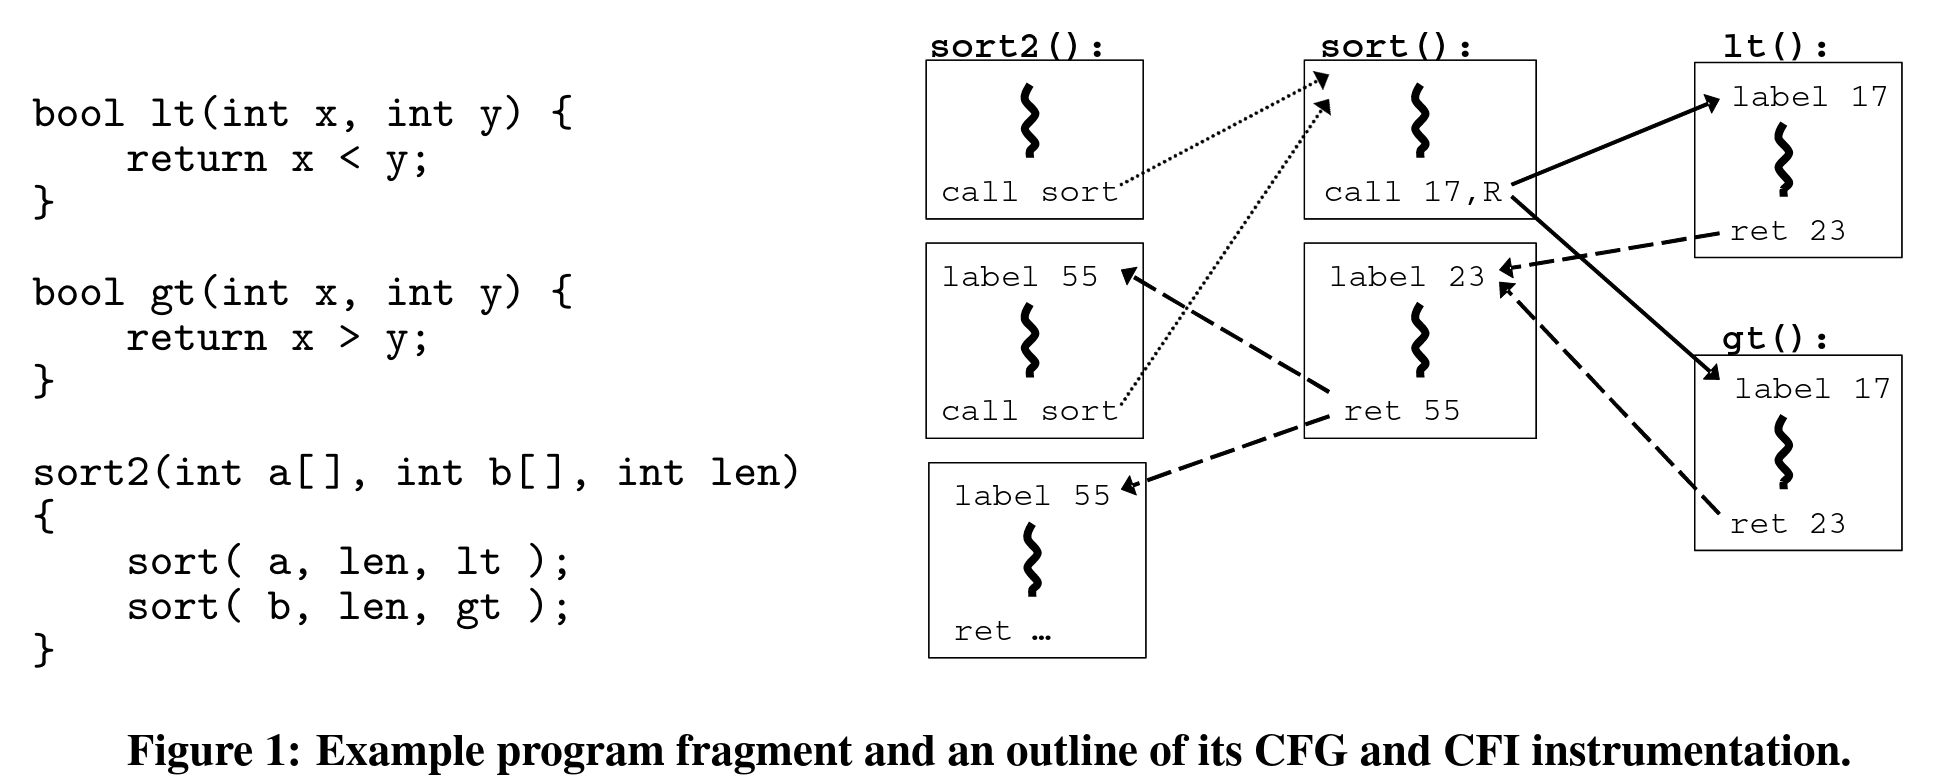
\includegraphics[width=0.7\textwidth]{../cfi/abadi-fig1}
\begin{itemize}
\item control flow graph
    \begin{itemize}
    \item nodes = blocks of code
    \item edges = \textit{potential jump/call}
    \end{itemize}
\item assigning labels: every in-edge needs to check same label at source
\end{itemize}
\imagecredit{figure from Abadi et al, ``Control-Flow Integrity: Principles, Implementations and Applications'' (CCS 2005)}
\end{frame}

 % FIXME: needs explanation of how labels assigned

\subsection{and function pointers}

\usetikzlibrary{arrows.meta}

\begin{frame}[fragile,label=tracking]{library-crossing CFGs}
\begin{tikzpicture}
\node[draw,very thick,label={north:main.c}] (mainc) {
\begin{lstlisting}[language=C++,style=script]
#include <png.h>
void ReadImageFromNetwork(
    png_structp libpng_handle,
    unsigned char *bytes,
    size_t size
) { ...  }

int main() {
    /* init libpng */
    png_structp libpng_handle = ...;
    /* tell libpng how to read image data */
    png_set_read_fn(
        libpng_handle, ...,
        ReadImageFromNetwork
    )
    ...
    /* extract "header" 
       information from image */
    png_get_IHDR(libpng_handle, ...)
    ...
}
\end{lstlisting}
};
\coordinate (base) at ([xshift=.5cm]mainc.north east);
\begin{scope}[shift=(base)]
    \tikzset{
        every node/.style={draw,align=left,font=\fontsize{10}{11}\tt\selectfont},
    }
    \node[draw,align=left,text width=1.25cm,anchor=north west] (main1) at (0,0) {
        main: \\
        ... \\
    };
    \node[draw,align=left] (set read) at (4, -1.5) {
        png\_set\_read\_fn: \\
        ... \\
        ...
    };

    \node[draw,align=left,text width=1.25cm,anchor=north west] (main2) at (0,-3) {
        ... \\
    };
    \draw[-Latex,very thick] (main1) -- (set read);
    \draw[-Latex,very thick] (set read) -- (main2);
    \node[draw,align=left] (ihdr) at (4, -4) {
        png\_get\_IHDR: \\
        ... \\
    };
    \node[draw,align=left] (readFromNet) at (5, -6) {
        ReadImage\\FromNetwork: \\
        ... 
    };
    \draw[-Latex,very thick] (main2) -- (ihdr);
    \draw[-Latex,very thick] (ihdr) -- (readFromNet);

    \begin{pgfonlayer}{bg}
    \draw[ultra thick,black!50,dotted,fill=blue!10] (-0.25,0.25) -- (1.9,0.25) -- (1.9,-5.2) -- (6.75,-5.2) --
        (6.75, -7) -- (-0.25,-7) -- cycle;
    \draw[ultra thick,black!50,dotted,fill=yellow!10] (2,-.5) -- (6.5,-.5) -- (6.5, -5) -- (2, -5) -- cycle;
    \end{pgfonlayer}
\end{scope}
\end{tikzpicture}
\end{frame}

\begin{frame}[fragile,label=imprecise]{CFGs will be imprecise}
\begin{lstlisting}[language=C++,style=smaller]
FunctionPtr p = functionA;
Example() {
  while (true) {
    ...
    if (SomethingComplicated()) {
      (*p)();
    } else if (SomethngElseComplicated()) {
      foo();
    }
    ...
  }
}
foo() {
  ...
  if (AnotherComplexThing()) {
    p = functionB;
  }
}
\end{lstlisting}
\begin{itemize}
\item can Example() call functionB()? probably not practical to tell
    \begin{itemize}
    \item need to make conservative `yes' guess
    \end{itemize}
\end{itemize}
\end{frame}


\subsection{finding function pointer values?}
\begin{frame}[fragile,label=fptrValues]{finding possible function pointer values?}
\begin{itemize}
\item given call using function pointers \\
how do we find the \textbf{legitimate} possible values?
\item one idea:
\end{itemize}
\begin{lstlisting}[language={},style=smaller,
    moredelim={**[is][\btHL<2-|handout:0>]{~2~}{~end~}},
]
for each fptr constant X: PossibleValues[X] = {X}
for each fptr ~2~variable X~end~:
    PossibleValues[X] = empty set
until PossibleValues stops changing:
    for each fptr assignment LHS=RHS:
        for ~2~each fptr variable/constant Y~end~
                ~2~that RHS could evaluate to~end~:
            PossibleValues[LHS] = Union(
                PossibleValues[LHS],
                PossibleValues[Y]
            )
\end{lstlisting}
\end{frame}




% FIXME:
\subsection{imprecision: unions, etc.}
\usetikzlibrary{arrows.meta}

\begin{frame}{labels aren't enough?}
\begin{tikzpicture}
\begin{scope}
\tikzset{
    every node/.style={align=left,draw,very thick,font=\tt\fontsize{11}{12}\selectfont},
}
\node (foo) at (0, 0){
    foo: \\
    ... \\
    check for label ??? \\
    call *p 
};

\node (bar) at (1, -5) {
    bar: \\
    ... \\
    check for label ??? \\
    call *p
};

\node (A) at (6, -2) { A: \\ label ??? };
\node (B) at (6, -3) { B: \\ label ??? };
\node (C) at (6, -4) { C: \\ label ??? };

\begin{scope}[-Latex,thick]
\draw (foo.south east) -- (A.west);
\draw (foo.south east) -- (C.west);
\draw (bar.south east) -- (B.west);
\draw (bar.south east) -- (C.west);
\end{scope}
\end{scope}
\begin{visibleenv}<2->
\node[align=left,draw=red,ultra thick,anchor=north west] at (8, 0) {
two possible fixes: \\
~ \\
make checks scan \\
for multiple labels \\
(more overhead) \\
~ \\
allow foo to call B \\
and bar to call A \\
(easier to attack)
};
\end{visibleenv}
\end{tikzpicture}
\end{frame}


\section{Clang's CFI implementation}
\begin{frame}{clang's CFI implementation}
\begin{itemize}
\item \url{https://clang.llvm.org/docs/ControlFlowIntegrity.html}
    \begin{itemize}
    \item \scriptsize also \url{https://www.usenix.org/conference/usenixsecurity14/technical-sessions/presentation/tice}
    \end{itemize}
\item only checks calls via VTables or function pointers
\item stable implementation requires libraries compiled with support
\item label information is placed in separate data structure
    \begin{itemize}
    \item \myemph<2>{looked up using function} or VTable addresses
    \end{itemize}
\item trick: keep functions in one region of memory
\end{itemize}
\end{frame}

\begin{frame}[fragile,label=indirectDiag]{clang idea for CFI indirect calls}
\begin{tikzpicture}
\node[draw, very thick, align=left] (dispatcher) {
\begin{lstlisting}[language=myasm,style=smaller]
start_funcs_with_two_string_args:
.align 8
compare_alpha:
  jmp real_compare_alpha
.align 8
run_command_with_arg:
  jmp real_run_command_with_arg
.align 8
print_two_strings:
  jmp real_print_two_strings
.align 8
move_file:
  jmp real_move_file
.align 8
compare_reverse_alpha:
  jmp real_compare_reverse_alpha
end_funcs_with_two_sting_args:
\end{lstlisting}
};
\begin{visibleenv}<1>
\node[align=left,draw=red,very thick,anchor=north west] at ([xshift=1cm]dispatcher.north east) {
functions of same type \\
placed together \\
~ \\
every func's address \\
is multiple of 8
};
\end{visibleenv}
\begin{visibleenv}<2>
\node[align=left,draw=red,very thick,anchor=north west] at ([xshift=0.5cm]dispatcher.north east) {
check pseudocode: \\
round fptr to multiple of 8 \\
\textbf{if} fptr < start or fptr > end: \\
\hspace{1cm} CRASH \\
allowed $\leftarrow$ [1,0,0,0,1] \\
\hspace{0.5cm} \textit{`mask' for compare funcs} \\
offset $\leftarrow$ fptr - start \\
\textbf{if} bit (offset/8) of allowed \\
\hspace{2.5cm}is not set: \\
\hspace{1cm} CRASH
};
\end{visibleenv}
\end{tikzpicture}
\end{frame}

\begin{frame}{clang idea for VTables}
\begin{itemize}
\item check VTable element address instead of function address
\item otherwise
    \begin{itemize}
    \item place all VTables for related classes together
    \item check start/end address for VTables
    \item bit mask indicating which VTable entries are okay for call
    \end{itemize}
\end{itemize}
\end{frame}


\section{Clang's CFI prevents?}
\begin{frame}[fragile,label=cfiPrevents]{CFI prevents?}
\begin{lstlisting}[language=C++,style=script]
class Foo { public: virtual void f() { } };
class Bar : public Foo { public: virtual void f() { g(1); } };
class Quux : public Foo { public: virtual void f() { } };
void g(int x) { if (x == 0) { danger(); } }
int h(int x) { return 0; }
int (*ptr)(int) = &h;
\end{lstlisting}
\begin{itemize}
\item with clang's CFI, which likely can end up calling \texttt{danger()}
      if an attacker can first write to arbitrary memory locations?
    \begin{itemize}
    \item A. \lstinline|(*ptr)(1);| 
    \item B. \lstinline|(*ptr)(0);| \only<2->{\myemph{if compiler thinks ptr set to g ever, yes; otherwise, no}}
    \item C. \lstinline|Foo *q = attacker_controlled(); q->f()| \only<2->{\myemph{can only call real f() methods; could call Bar::f() but how to change g's arg?}}
    \item D. \lstinline|Quux *q = attacker_controlled(); q->f()| \only<2->{\myemph{can only call real f() methods of Quux and subclasses, so can't even call Bar::f()}}
    \item E. none of these
    \end{itemize}
\end{itemize}
\end{frame}


\subsection{problems with dynamically loaded code}
\begin{frame}{CFI: dynamically loaded libraries?}
    \begin{itemize}
    \item what about dynamically loaded libraries\ldots
    \item problem: precomputed control flow graph now invalid
    \end{itemize}
\end{frame}


\section{Intel's `CFI'}
\begin{frame}{Intel hardware CFI support}
    \begin{itemize}
    \item Intel adds `endbr64' instruction
    \item special NOP instruction that acts as a label
    \item means: only one label for everything
        \begin{itemize}
        \item prevents gadgets from existing
        \end{itemize}
    \vspace{.5cm}
    \item ``Control Flow Enforcement'': if enabled \\
        computed jump to non-endbr64 triggers segfault-like error
    \vspace{.5cm}
    \item ARM has similar feature called Branch Target Identification
    \end{itemize}
\end{frame}


\section{authenticated pointers}

\begin{frame}[fragile,label=authPtr1]{authenticated pointers (1)}
\begin{lstlisting}[language={},style=smaller]
some_function:
    authentication_code <- MAC(
        secret key, 
        return address
    )
    ... dangerous function code ...
    assert(authenication_code ==
        MAC(secret key, return addres))
    jump to return address
\end{lstlisting}
\end{frame}

\begin{frame}[fragile,label=authPtr2]{authenticated pointers (2)}
\begin{lstlisting}[language={},style=smaller]
some_function:
    authentication_code <- MAC(
        secret key,
        stack pointer, 
        return address
    )
    ... dangerous function code ...
    assert(authenication_code ==
        MAC(secret key, stack pointer, return address))
    jump to return address
\end{lstlisting}
\end{frame}


\begin{frame}[fragile,label=authPtr3]{authenticated pointers (3)}
\begin{lstlisting}[language={},style=smaller]
some_function:
    return address <- encode(
        secret key,
        stack pointer, 
        return address
    )
    ... dangerous function code ...
    return address <- decode_or_crash(
        secret key,
        stack pointer, 
        return address
    )
    jump to return address
\end{lstlisting}
\end{frame}

\begin{frame}[fragile,label=authPtr4]{authenticated pointers (4)}
\begin{lstlisting}[language={},style=smaller]
some_vtable[index] <- encrypt(
    secret key,
    label,
    address of some of function
)
... dangerous code ...
function pointer <- decrypt(
    secret key,
    label,
    object->vtable[index]
)
call function pointer
\end{lstlisting}
\end{frame}

\begin{frame}{ARM authenticated pointers}
    \begin{itemize}
    \item ARM64 implements this idea with:
    \vspace{.5cm}
    \item secret key kept in a special register (hard to leak to attacker)
    \item authentication code placed in upper pointer bits
        \begin{itemize}
        \item makes pointer temporarily invalid
        \item can't ``accidentally'' use authenticated pointer without verifying authentication code first
        \end{itemize}
    \end{itemize}
\end{frame}

\begin{frame}[fragile]{authenticated pointer layout}
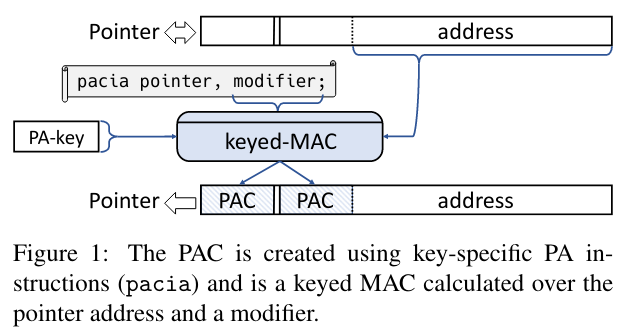
\includegraphics[width=\textwidth]{../cfi/arm-enc-ptr-fig}
\imagecredit{Liljestrand et al, ``PAC it up: Towards Pointer Integrity using ARM Pointer Authentication''}
\end{frame}

\begin{frame}{authentication keys}
    \begin{itemize}
    \item processes can have multiple authentication keys active
    \item easy to use separate keys for
        \begin{itemize}
        \item return address pointers
        \item function pointers
        \item any pointers to data
        \end{itemize}
    \item authentication keys are in special registers --- need OS to read/set
    \vspace{.5cm}
    \item also can ``mix'' in extra info like stack pointer
    \end{itemize}
\end{frame}

\begin{frame}{pointer authentication use}
    \begin{itemize}
    \item commonly enabled on ARM64 for return addreses
    \vspace{.25cm}
    \item otherwise:
    \item on ARM64 OS X --- used by OS X
        \begin{itemize}
        \item two different compiler `architectures': arm64, arm64e
        \item can't use arm64e libraries in arm64 program or vice-versa
        \end{itemize}
    \item proposals to use on Linux in global offset table, etc.
        \begin{itemize}
        \item GNU Linux linker option -z pac-plt; unclear if used `for real'
        \end{itemize}
    \end{itemize}
\end{frame}

\begin{frame}[fragile]{macOS PAC for apple code}
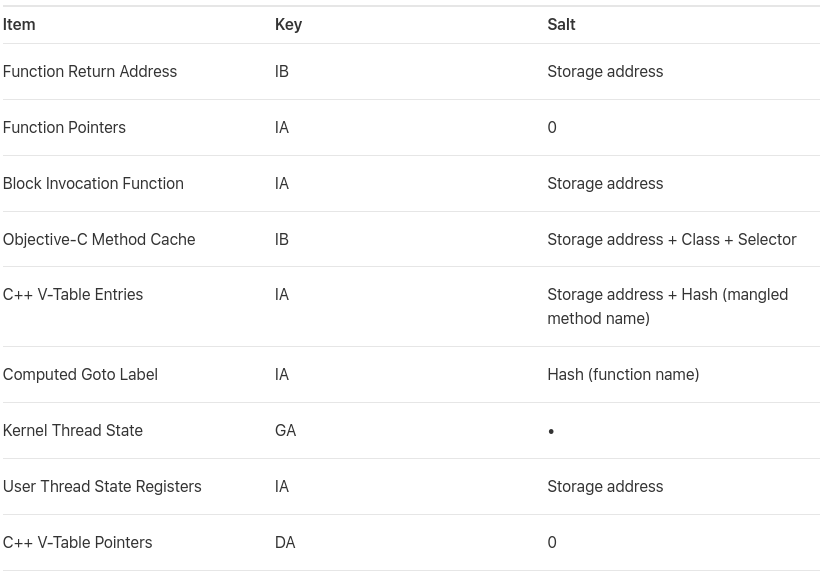
\includegraphics[height=0.9\textheight]{../cfi/apple-pac-usage}
\imagecredit{\url{https://support.apple.com/en-il/guide/security/sec8b776536b/1/web/1}}
\end{frame}

\begin{frame}{macOS PAC}
    \begin{itemize}
    \item `new' `preview' architecture in compiter
    \item seems to be used internally by Apple
    \item doesn't appear easily available/supported for others
    \item incompatible with `old' libraries
    \end{itemize}
\end{frame}

\begin{frame}{PAC bypasses}
    \begin{itemize}
    \item have been exploits in spite of PAC in iOS kernel
    \vspace{.5cm}
    \item only certain code pointers authenticated
        \begin{itemize}
        \item too expensive to authenticate all pointers
        \end{itemize}
    \item changing unsigned pointer values just before signed 
        \begin{itemize}
        \item get context switch to occur at just the right time
        \item modify pointer value in saved context
        \end{itemize}
    \item code that signs pointers they shouldn't
        \begin{itemize}
        \item changing pointer without crashing if old pointer invalid
        \end{itemize}
    \item `gadgets' that allow brute-forcing MAC tag
        \begin{itemize}
        \item not enough space in pointers for non-brute-forceable tag
        \end{itemize}
    \end{itemize}
\end{frame}

% FIXME



\section{backup slides}
\begin{frame}{backup slides}
\end{frame}
\section{baggy bounds checking}

\begin{frame}{research example (2009)}
    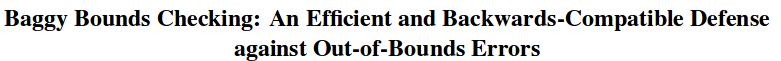
\includegraphics[width=\textwidth]{../bounds/baggy-bounds-title}
\end{frame}

\begin{frame}[fragile,label=lookupTable]{baggy bounds checking idea}
    \begin{itemize}
        \item giant lookup table --- one entry for every 16 bytes of memory
        \item table indicates start of object allocated here
        \item check pointer arithmetic:
    \end{itemize}
\begin{lstlisting}
char p = str[i];
/* becomes: */
CHECK(START_OF[str / 16] == START_OF[&str[i] / 16]);
char p = str[i];
\end{lstlisting}
\end{frame}




\subsection{trick for good performance}

\begin{frame}[fragile,label=baggyBoundsTrick]{baggy bounds trick}
\lstset{language=C,style=small}
    \begin{itemize}
        \item table of pointers to starting locations would be huge
        \item add some restrictions:
            \begin{itemize}
            \item all object sizes are powers of two
            \item all object starting addresses are a multiple of their size
            \end{itemize}
        \item then, table contains size info only:
            \begin{itemize}
            \item table contains $i$, size is $2^i$ bytes:
            \end{itemize}
    \end{itemize}
\begin{lstlisting}
char *GetStartOfObject(char *pointer) {
    return pointer & ~(1 << TABLE[pointer / 16] - 1);
    /* pointer bitwise-and 2^(table entry) - 1 */
    /* clear lower (table entry) bits  of pointer */
}
\end{lstlisting}
\end{frame}



\subsection{the lookup table}
\usetikzlibrary{fit,matrix}

\tikzset{
    stackBox/.style={very thick},
    allocBox/.style={dashed,very thick,fill=blue!20},
    onStack/.style={thick},
    frameOne/.style={fill=blue!15},
    frameTwo/.style={fill=red!15},
    markLine/.style={blue!50!black},
    markLineB/.style={red!90!black},
    hiLine/.style={red!90!black},
}
\begin{frame}<1-6>[fragile,label=lkpTble]{allocations and lookup table}
    \begin{tikzpicture}
        \draw[onStack] (0, 0) rectangle (4, -7);
        \draw[allocBox] (0, 0) rectangle (4, -0.4);
        \draw[stackBox] (0, 0) rectangle (4, -0.5);
        \draw[allocBox] (0, -0.5) rectangle (4, -0.8);
        \draw[stackBox] (0, -0.5) rectangle (4, -1.0);
        \draw[allocBox] (0, -1) rectangle (4, -1.9);
        \draw[stackBox] (0, -1) rectangle (4, -2);
        \draw[allocBox] (0, -2) rectangle (4, -2.4);
        \draw[stackBox] (0, -2) rectangle (4, -2.5);
        \draw[allocBox] (0, -2.5) rectangle (4, -2.7);
        \draw[stackBox] (0, -2.5) rectangle (4, -3);
        \draw[stackBox] (0, -3) rectangle (4, -4);
        \draw[allocBox] (0, -4) rectangle (4, -5.2);
        \draw[stackBox] (0, -4) rectangle (4, -6);

        \begin{visibleenv}<1->
            \node[anchor=north west,align=left] at (9, 0) {
                object allocated in \\ \myemph<1>{power-of-two `slots'}
            };
        \end{visibleenv}
        \begin{visibleenv}<2->
            \matrix[tight matrix,
                nodes={text width=1cm,font=\small\tt},anchor=north west,label={north:table}] (tbl) at (7, -1) {
                $2^4$ \\ $2^4$  \\ $2^5$ \\ $2^5$ \\ $2^4$ \\ $2^4$ \\
                $0$ \\ $0$ \\
                $2^6$ \\ $2^6$ \\ $2^6$ \\ $2^6$ \\
            };
            \begin{scope}[thick,dotted,-Latex]
            \draw (4, -.25) -- (tbl-1-1.west);
            \draw (4, -.75) -- (tbl-2-1.west);
            \draw (4, -1.25) -- (tbl-3-1.west);
            \draw (4, -1.75) -- (tbl-4-1.west);
            \draw (4, -2.25) -- (tbl-5-1.west);
            \draw (4, -2.75) -- (tbl-6-1.west);
            \draw (4, -3.25) -- (tbl-7-1.west);
            \draw (4, -3.75) -- (tbl-8-1.west);
            \draw (4, -4.25) -- (tbl-9-1.west);
            \end{scope}
        \end{visibleenv}
        \begin{visibleenv}<3>
            \draw[ultra thick,red] (0, -1) rectangle (4, -2);
            \node[draw,ultra thick,red,inner sep=0mm,fit=(tbl-3-1) (tbl-4-1)] {};
            \draw[ultra thick,blue] (0, -4) rectangle (4, -6);
            \node[draw,ultra thick,blue,inner sep=0mm,fit=(tbl-9-1) (tbl-12-1)] {};
        \end{visibleenv}
        \begin{visibleenv}<3->
            \node[anchor=north west,align=left] at (9, -2) {
                table stores sizes \\
                \myemph{for each 16 bytes}
            };
        \end{visibleenv}
        \begin{visibleenv}<4>
            \draw[ultra thick,red] (0, -3) rectangle (4, -4);
            \node[draw,ultra thick,red,inner sep=0mm,fit=(tbl-7-1) (tbl-8-1)] {};
        \end{visibleenv}
        \begin{visibleenv}<4->
            \node[anchor=north west,align=left] at (9, -3.5) {
                addresses \textbf<4>{multiples of size} \\
                (may \myemph{require padding})
            };
        \end{visibleenv}
        \begin{pgfonlayer}{bg}
        \begin{visibleenv}<5>
            \fill[red!30] (0, -5.2) rectangle (4, -6.);
            \fill[red!30] (0, -2.7) rectangle (4, -3.);
            \fill[red!30] (0, -1.9) rectangle (4, -2.);
            \fill[red!30] (0, -2.4) rectangle (4, -2.5);
            \fill[red!30] (0, -0.8) rectangle (4, -1.);
            \fill[red!30] (0, -0.4) rectangle (4, -0.5);
        \end{visibleenv}
        \end{pgfonlayer}
        \begin{visibleenv}<5->
            \node[anchor=north west,align=left] at (9, -5.5) {
                sizes are \textbf<5>{powers of two} \\
                (may \myemph{require padding})
            };
        \end{visibleenv}
    \end{tikzpicture}
\end{frame}

\begin{frame}[fragile,label=managing]{managing the table}
    \begin{itemize}
        \item not just done \texttt{malloc()/new}
        \item also for stack allocations:
    \end{itemize}
    \begin{lstlisting}[style=small,language=C]
void vulnerable() {
    char buffer[100];
    gets(vulnerable);
}
\end{lstlisting}
    \begin{tikzpicture}[remember picture, overlay]
        \node[anchor=north east] at ([xshift=-.25cm, yshift=-1cm]current page.north east) {
    \begin{lstlisting}[style=small,language=myasm]
vulnerable:
  // make %rsp a multiple
  // of 128 (2^7) 
  andq $0xFFFFFFFFFFFFFF80, %rsp
  // allocate 128 bytes
  subq $0x80, %rsp
  // rax <- rsp / 16
  movq $rsp, %rax
  shrq $4, %rax
  movb $7, TABLE(%rax)
  movb $7, TABLE+1(%rax)
  ...
  movq %rsp, %rdi
  call gets
  ret
\end{lstlisting}
};
    \end{tikzpicture}
\end{frame}

\begin{frame}[fragile,label=sparseLookup]{sparse lookup table}
    \begin{tikzpicture}
        \node[anchor=south] at (3.5, 3) {lookup table};
        \draw[stackBox] (0, 3) rectangle (7, -3);
        \draw[pattern color=red,pattern=north west lines,onStack] (0, -3) rectangle (7, -1.5)
            node[midway,fill=white,align=center] {unallocated memory (segfault) };
        \draw[fill=green,onStack] (0, -1.5) rectangle (7, .2)
            node[midway] { allocated part of table };
        \draw[pattern color=red,pattern=north west lines,onStack] (0, .20) rectangle (7, 1.3)
            node[midway,fill=white,align=center] {unallocated memory (segfault) };
        \draw[fill=green,onStack] (0, 1.3) rectangle (7, 1.6);
        \draw[pattern color=red,pattern=north west lines,onStack] (0, 1.6) rectangle (7, 2.3);
        \draw[fill=green,onStack] (0, 2.3) rectangle (7, 3)
            node[midway] { allocated part of table };
    \end{tikzpicture}
\end{frame}



\subsection{aside: binary translation}
% From 20170123
\usetikzlibrary{positioning}

\begin{frame}{binary translation}
    \begin{itemize}
    \item compile assembly to new assembly
    \vspace{1cm}
    \item works without instruction set support
    \item early versions of VMWare on x86 (before x86 added virtualisation support)
    \item can be used to run one platform on another
    \end{itemize}
\end{frame}

\begin{frame}[fragile,label=binTransIdea]{binary translation idea}
\lstset{
    language=myasm,
    style=small,
    morekeywords={movq,addss,subss}
}
\begin{tikzpicture}
\tikzset{
    code/.style={inner sep=0mm,align=left},
    hiOn/.style={alt=#1{rounded corners,fill=green,fill opacity=0.3,text opacity=1.0}{}},
    markOn/.style={alt=#1{rounded corners,draw,thick}{}},
}
\node[code,markOn=<2>,hiOn=<3>] (bb1) {
\begin{lstlisting}
0x40FE00: addq %rax, %rbx
movq 14(%r14,4), %rdx
addss %xmm0, (%rdx)
...
0x40FE3A: jne 0x40F404
\end{lstlisting}
};
\node[right=.25cm of bb1,visible on=<2>,align=left] {
    divide machine code \\
    into \textit{basic blocks} \\
    (= ``straight-line'' code) \\
    (= code till \\ 
    jump/call/etc.)
};
\node[code,right=.25cm of bb1,visible on=<3>] (bb1New) {
generated code: \\
\begin{lstlisting}
// addq %rax, %rbx
movq rax_location, %rdi
movq rbx_location, %rsi
call checked_addq
movq %rax, rax_location
...
// jne 0x40F404
... // get CCs 
je do_jne
movq $0x40FE3F, %rdi
jmp translate_and_run
do_jne:
movq $0x40F404, %rdi
jmp translate_and_run
\end{lstlisting}
};
\node[code,markOn=<2>,anchor=north west] (bb2) at (bb1.south west){
\begin{lstlisting}
subss %xmm0, 4(%rdx)
...
je 0x40F543
\end{lstlisting}
};
\node[code,markOn=<2>,anchor=north west] (bb3) at (bb2.south west){
\begin{lstlisting}
ret
\end{lstlisting}
};
\end{tikzpicture}
\end{frame}

\begin{frame}[fragile,label=binTransIdea2]{a binary translation idea}
    \begin{itemize}
    \item convert whole \textit{basic blocks}
        \begin{itemize}
        \item code upto branch/jump/call
        \end{itemize}
    \item end with call to {\tt translate\_and\_run}
        \begin{itemize}
        \item compute new \myemph{simulated PC} address to pass to call
        \end{itemize}
    \end{itemize}
\end{frame}

\begin{frame}[fragile,label=binTransIdea3]{making binary translation fast}
    \lstset{style=small,language=myasm,morekeywords={movq}}
    \begin{itemize}
    \item cache converted code
        \begin{itemize}
        \item {\tt translate\_and\_run} checks cache first
        \end{itemize}
    \item patch calls to {\tt translate\_and\_run} to refer directly to cached code
    \item do something more clever than \lstinline|movq rax_location, ...|
        \begin{itemize}
        \item map (some) registers to registers, not memory
        \end{itemize}
    \item ends up being ``just-in-time'' compiler
    \end{itemize}
\end{frame}


\begin{frame}{binary translation? really?}
    \begin{itemize}
    \item early VMWare: for instructions without hardware virtualization support
        \begin{itemize}
        \item only needed for little bits of OS code
        \end{itemize}
    \item used by Apple to handle changing CPU designs
    \item Rosetta 2: run Intel on ARM (current)
    \item Rosetta: run Power PC on Intel (2005--2011)
    \item Mac 68k emulator: Run Motorola 680x0 on Power PC (1994--2005)
    \end{itemize}
\end{frame}




\end{document}
